\documentclass[12pt]{article}
\usepackage{amsmath, amssymb, amsthm, tikz, pgfplots}
\usepackage{geometry, enumitem, mdframed, xcolor}
\geometry{margin=1in}

% Custom environments
\newtheorem{definition}{Definition}
\newtheorem{theorem}{Theorem}
\newtheorem{method}{Method}
\newtheorem{example}{Example}
\newmdenv[linecolor=blue,linewidth=2pt]{keypoint}
\newmdenv[linecolor=red,linewidth=2pt]{warning}
\newmdenv[linecolor=green,linewidth=2pt]{insight}

\title{ODE Lesson 9: Direction Fields and Isoclines - Visualizing ODE Solutions}
\author{ODE 1 - Prof. Adi Ditkowski}
\date{}

\begin{document}
\maketitle

\section{Introduction to Direction Fields}

\begin{definition}[Direction Field]
For a first-order ODE $\frac{dy}{dx} = f(x,y)$, the \textbf{direction field} (or slope field) is a graphical representation where at each point $(x,y)$ in the plane, we draw a short line segment with slope $f(x,y)$.
\end{definition}

\begin{keypoint}
Direction fields provide a complete qualitative picture of all solutions without solving the ODE!
\end{keypoint}

\section{Construction Algorithm}

\begin{method}[Creating Direction Fields]
\begin{enumerate}
    \item Choose a grid of points $(x_i, y_j)$ in the region of interest
    \item At each point, calculate the slope $m_{ij} = f(x_i, y_j)$
    \item Draw a short line segment centered at $(x_i, y_j)$ with slope $m_{ij}$
    \item Keep all segments approximately the same length
\end{enumerate}
\end{method}

\section{Isoclines}

\begin{definition}[Isocline]
An \textbf{isocline} for slope $c$ is the set of all points where $f(x,y) = c$.
\end{definition}

\begin{insight}
Isoclines dramatically simplify direction field construction! Along each isocline, all direction segments have the same slope.
\end{insight}

\begin{example}[Finding Isoclines]
For $\frac{dy}{dx} = 2x - y$:
\begin{itemize}
    \item Isocline for slope $0$: $2x - y = 0 \Rightarrow y = 2x$
    \item Isocline for slope $1$: $2x - y = 1 \Rightarrow y = 2x - 1$
    \item Isocline for slope $-1$: $2x - y = -1 \Rightarrow y = 2x + 1$
\end{itemize}
\end{example}

\section{Special Features}

\subsection{Equilibrium Points}

\begin{definition}[Equilibrium Point]
A point $(x_0, y_0)$ where $f(x_0, y_0) = 0$ is an \textbf{equilibrium point}. Solutions starting at equilibria remain constant.
\end{definition}

\subsection{Nullclines}

\begin{definition}[Nullcline]
The \textbf{nullcline} is the isocline where $f(x,y) = 0$, consisting of all equilibrium points and curves of horizontal tangents.
\end{definition}

\begin{warning}
Do not confuse isoclines with solution curves! Isoclines show where slopes are constant; solution curves follow the changing slopes.
\end{warning}

\section{Sketching Solution Curves}

\begin{method}[Drawing Solutions from Direction Fields]
\begin{enumerate}
    \item Choose an initial point $(x_0, y_0)$
    \item Draw a smooth curve that is tangent to the direction segment at every point
    \item The curve should "flow" with the field, never crossing arrows at wrong angles
    \item Pay special attention near equilibria and nullclines
\end{enumerate}
\end{method}

\section{Qualitative Analysis Features}

\begin{theorem}[Direction Field Properties]
From a direction field, we can determine:
\begin{itemize}
    \item Location and type of equilibria
    \item Stability of equilibria (attracting/repelling)
    \item Existence of separatrices
    \item Long-term behavior of solutions
    \item Regions of monotonic behavior
\end{itemize}
\end{theorem}

\section{Examples with Direction Fields}

\begin{example}[Linear ODE: $\frac{dy}{dx} = x - y$]
\begin{center}
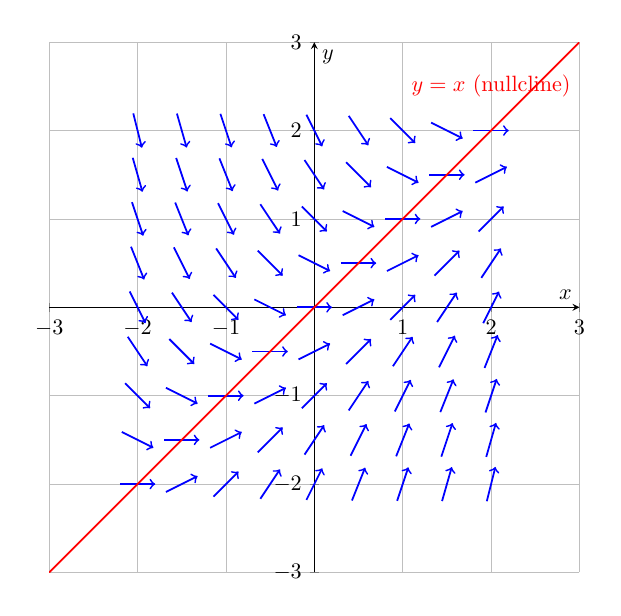
\begin{tikzpicture}[scale=0.8]
\begin{axis}[
    xlabel={$x$},
    ylabel={$y$},
    xmin=-3, xmax=3,
    ymin=-3, ymax=3,
    axis lines=middle,
    grid=major,
    width=10cm,
    height=10cm,
]
% Direction field
\foreach \x in {-2,-1.5,...,2} {
    \foreach \y in {-2,-1.5,...,2} {
        \edef\slope{(\x-\y)}
        \edef\norm{sqrt(1+(\slope)^2)}
        \addplot[blue, thick, ->] coordinates {
            (\x-0.2/\norm, \y-0.2*\slope/\norm)
            (\x+0.2/\norm, \y+0.2*\slope/\norm)
        };
    }
}
% Nullcline y = x
\addplot[red, thick, domain=-3:3] {x};
\node[red] at (axis cs:2,2.5) {$y = x$ (nullcline)};
\end{axis}
\end{tikzpicture}
\end{center}
\end{example}

\section{Exam Strategy}

\begin{keypoint}
Prof. Ditkowski's Common Questions:
\begin{enumerate}
    \item Sketch the direction field for a given ODE
    \item Identify all equilibria from a direction field
    \item Draw solution curves through specific points
    \item Determine long-term behavior without solving
    \item Find and classify isoclines
\end{enumerate}
\end{keypoint}

\section{Memory Aids}

\begin{center}
\textbf{Direction Field Analysis Steps:}\\
\textbf{D}raw grid points\\
\textbf{I}dentify isoclines\\
\textbf{R}ecognize equilibria\\
\textbf{E}valuate slopes\\
\textbf{C}onstruct solution curves\\
\textbf{T}rack long-term behavior
\end{center}

\end{document}